\section{Auswertung}
\label{sec:Auswertung}
Für die Auswertung der Messwerte wird im Folgenden der Mittelwert immer als
\begin{equation}
  \bar{x} = \frac{1}{N}\sum_{i=1}^{N} x_{i}
\end{equation}
berechnet und die Standardabweichung mit
\begin{equation}
  \Delta\bar{x} = \frac{\sigma}{\sqrt{N}} = \sqrt{\frac{1}{N(N-1)}\sum_{i=1}^{N} (x_{i} - \bar{x})^2}.
\end{equation}

Für die Bestimmung der Grenzspannungen werden die Messwerte aus den Tabellen \ref{tab:gelb},
\ref{tab:gruen}, \ref{tab:blaugruen}, \ref{tab:violett1} und \ref{tab:violett2} in den Abbildungen 
\ref{fig:gelb}, \ref{fig:gruen}, \ref{fig:blaugruen}, \ref{fig:violett1} und \ref{fig:violett2} aufgetragen.
Weiterhin wird eine lineare Regression der Form
\begin{equation}
  \sqrt{I} = a\cdot U + b
\end{equation}
vorgenommen. Die Grenzspannung $U_\text{G}$ ist die Nullstelle dieser Geraden und berechnet sich nach
\begin{equation}
  U_\text{G} = -\frac{b}{a}.
\end{equation}

Der Fehler errechnet sich dabei mittels Gaußscher Fehlerfortpflanzung
\begin{equation}
  \Delta U_\text{G} = \sqrt{\frac{(\Delta b)^{2}}{a^{2}} + \frac{b^{2} (\Delta a)^{2}}{a^{4}}}.
\end{equation}
Die zu den einzelnen Wellenlängen gehörigen Regressionskoeffizienten sowie die Grenzspannungen werden 
in Tabelle \ref{tab:grenz} abgebildet.

%GELB
\begin{table}[H]
  \centering
  \caption{Messwerte von $U$ und $I$ bei gelbem Licht mit Wellenlänge $\lambda = \SI{578.05}{\nano\meter}$.}
  \label{tab:gelb}
  \begin{tabular}{S[table-format=1.2] S[table-format=1.3]}
    \toprule
    {$U \:/\: \si{\volt}$} & {$I \:/\: \si{\nano\ampere}$}\\
    \midrule
    0.01 &   0.360 \\
    0.05 &   0.330 \\
    0.10 &   0.280 \\
    0.15 &   0.220 \\
    0.20 &   0.170 \\
    0.25 &   0.120 \\
    0.30 &   0.084 \\
    0.35 &   0.055 \\
    0.40 &   0.030 \\
    0.45 &   0.015 \\
    0.50 &   0.005 \\
  \end{tabular}
\end{table}

\begin{figure}[H]
  \centering
  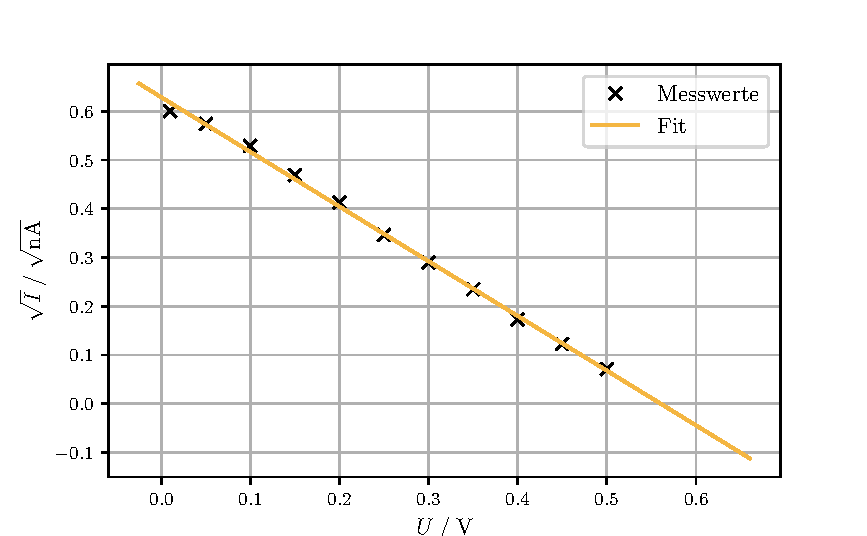
\includegraphics{gelb.pdf}
  \caption{Messwerte der gelben Spektrallinie mit $\lambda = \SI{578.05}{\nano\meter}$ sowie die dazugehörige Regressionsgerade.}
  \label{fig:gelb}
\end{figure}

%GRÜN

\begin{table}[H]
  \centering
  \caption{Messwerte von $U$ und $I$ bei grünem Licht mit Wellenlänge $\lambda = \SI{546}{\nano\meter}$.}
  \label{tab:gruen}
  \begin{tabular}{S[table-format=1.2] S[table-format=1.3]}
    \toprule
    {$U \:/\: \si{\volt}$} & {$I \:/\: \si{\nano\ampere}$}\\
    \midrule
    0.50  &  0.005 \\
    0.45  &  0.014 \\
    0.40  &  0.028 \\
    0.35  &  0.048 \\
    0.30  &  0.076 \\
    0.25  &  0.100 \\
    0.20  &  0.140 \\
    0.15  &  0.170 \\
    0.10  &  0.200 \\
    0.05  &  0.240 \\
    0.02  &  0.270 \\
  \end{tabular}
\end{table}

\begin{figure}[H]
  \centering
  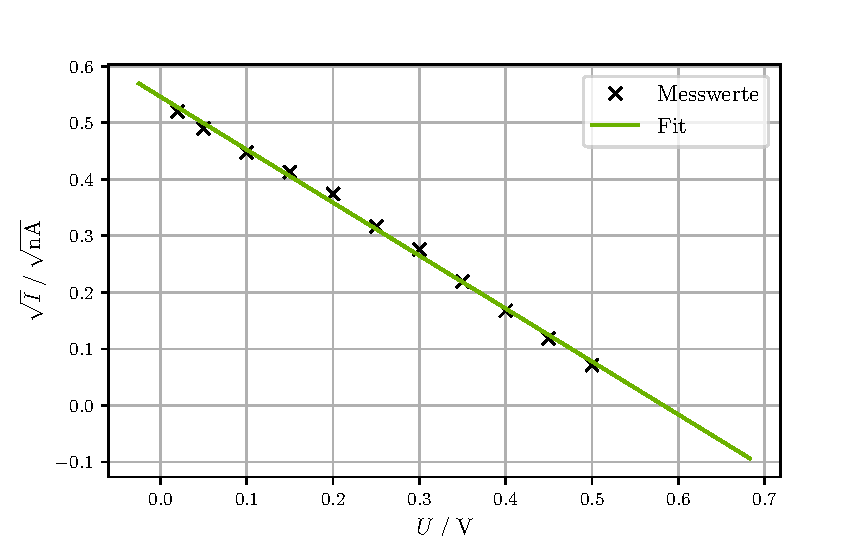
\includegraphics{gruen.pdf}
  \caption{Messwerte der grünen Spektrallinie mit $\lambda = \SI{546}{\nano\meter}$ sowie die dazugehörige Regressionsgerade.}
  \label{fig:gruen}
\end{figure}

%BLAUGRUEN
\begin{table}[H]
  \centering
  \caption{Messwerte von $U$ und $I$ bei blaugrünem Licht mit Wellenlänge $\lambda = \SI{491.6}{\nano\meter}$.}
  \label{tab:blaugruen}
  \begin{tabular}{S[table-format=1.2] S[table-format=1.3]}
    \toprule
    {$U \:/\: \si{\volt}$} & {$I \:/\: \si{\nano\ampere}$}\\
    \midrule
    0.50  &  0.005 \\
    0.45  &  0.008 \\
    0.40  &  0.011 \\
    0.35  &  0.014 \\
    0.30  &  0.018 \\
    0.25  &  0.022 \\
    0.20  &  0.026 \\
    0.15  &  0.028 \\
    0.10  &  0.033 \\
    0.05  &  0.036 \\
    0.02  &  0.039 \\
  \end{tabular}
\end{table}

\begin{figure}[H]
  \centering
  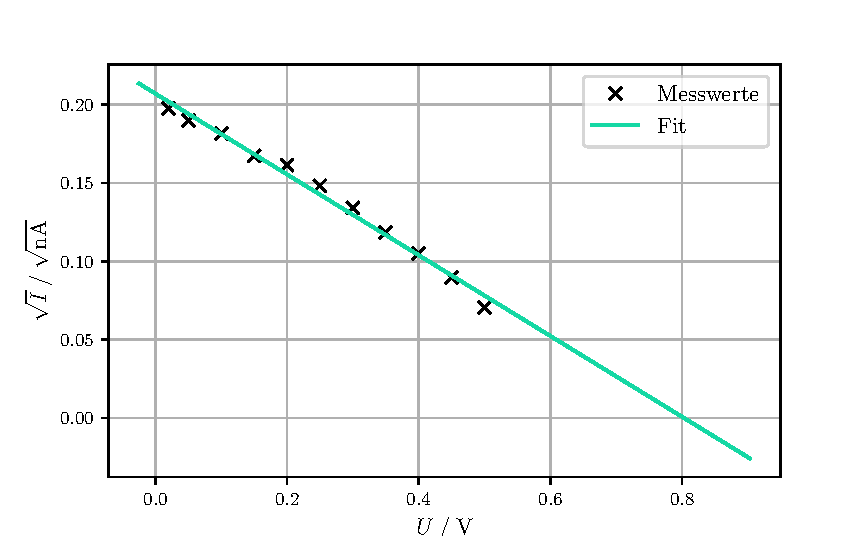
\includegraphics{blaugruen.pdf}
  \caption{Messwerte der blaugrünen Spektrallinie mit $\lambda = \SI{491.6}{\nano\meter}$ sowie die dazugehörige Regressionsgerade.}
  \label{fig:blaugruen}
\end{figure}



%VIOLETT1
\begin{table}[H]
  \centering
  \caption{Messwerte von $U$ und $I$ bei violettem Licht mit Wellenlänge $\lambda = \SI{435.25}{\nano\meter}$.}
  \label{tab:violett1}
  \begin{tabular}{S[table-format=1.2] S[table-format=1.3]}
    \toprule
    {$U \:/\: \si{\volt}$} & {$I \:/\: \si{\nano\ampere}$}\\
    \midrule
    0.90 &   0.038 \\
    0.80 &   0.077 \\
    0.70 &   0.120 \\
    0.60 &   0.200 \\
    0.50 &   0.300 \\
    0.40 &   0.400 \\
    0.30 &   0.520 \\
    0.20 &   0.620 \\
    0.10 &   0.730 \\
    0.02 &   0.840 \\
  \end{tabular}
\end{table}

\begin{figure}[H]
  \centering
  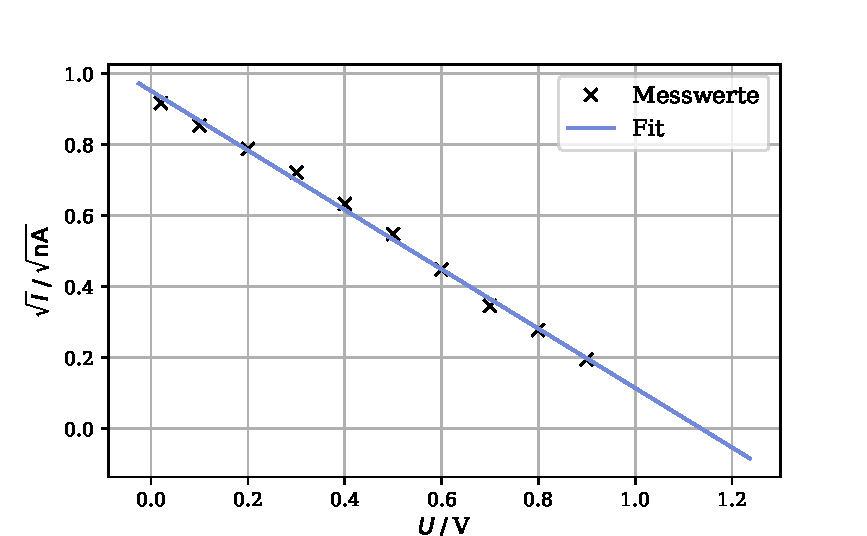
\includegraphics{violett1.pdf}
  \caption{Messwerte der ersten violetten Spektrallinie mit $\lambda = \SI{435.25}{\nano\meter}$ sowie die dazugehörige Regressionsgerade.}
  \label{fig:violett1}
\end{figure}

%VIOLETT2
\begin{table}[H]
  \centering
  \caption{Messwerte von $U$ und $I$ bei violettem Licht mit Wellenlänge $\lambda = \SI{406.25}{\nano\meter}$.}
  \label{tab:violett2}
  \begin{tabular}{S[table-format=1.2] S[table-format=1.3]}
    \toprule
    {$U \:/\: \si{\volt}$} & {$I \:/\: \si{\nano\ampere}$}\\
    \midrule
    0.02  &  0.580 \\
    0.12  &  0.500 \\
    0.24  &  0.400 \\
    0.36  &  0.320 \\
    0.48  &  0.240 \\
    0.60  &  0.170 \\
    0.72  &  0.120 \\
    0.84  &  0.074 \\
    0.96  &  0.042 \\
    1.08  &  0.018 \\
    1.20  &  0.004 \\
  \end{tabular}
\end{table}

\begin{figure}[H]
  \centering
  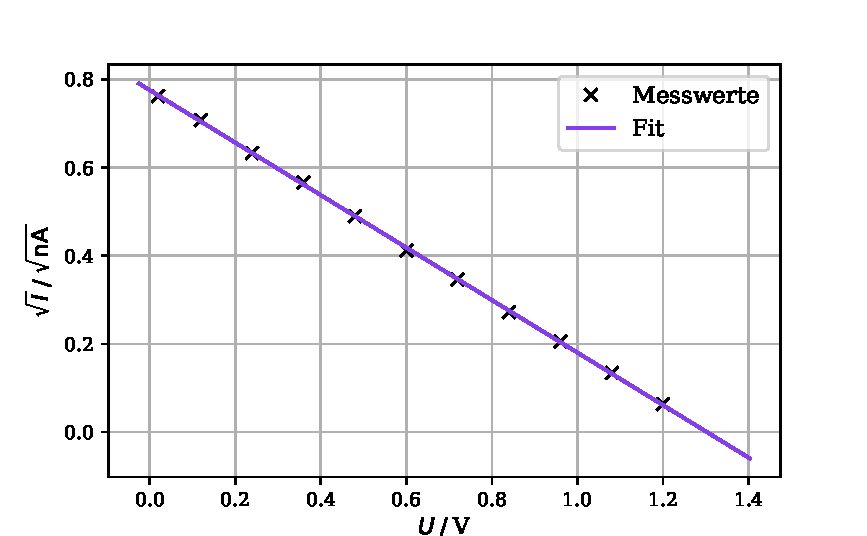
\includegraphics{violett2.pdf}
  \caption{Messwerte der zweiten violetten Spektrallinie mit $\lambda = \SI{406.25}{\nano\meter}$ sowie die dazugehörige Regressionsgerade.}
  \label{fig:violett2}
\end{figure}

%GRENZ
\begin{table}[H]
  \centering
  \caption{Den Spektrallinien zugehörigen Regressionskoeffizienten und damit berechneten Grenzspannungen aus den Abbildungen \ref{fig:gelb}, \ref{fig:gruen},
  \ref{fig:blaugruen}, \ref{fig:violett1} und \ref{fig:violett2}.}
  \label{tab:grenz}
  \begin{tabular}{c S[table-format=3.2]
    S[table-format=2.3]@{${}\pm{}$}S[table-format=1.3]
    S[table-format=1.3]@{${}\pm{}$}S[table-format=1.3]
    S[table-format=1.3]@{${}\pm{}$}S[table-format=1.3]}
    \toprule
    {Farbe} & {$\lambda \:/\: \si{\nano\meter}$} & \multicolumn{2}{c}{$a \:/\: \sqrt{\si{\ampere\per\volt}}$} &
    \multicolumn{2}{c}{$b \:/\: \sqrt{\si{\ampere}}$} & \multicolumn{2}{c}{$U_\text{G} \:/\: \si{\volt}$}\\
    \midrule
    gelb          &   578.05   &   -1.122  &  0.017    &    0.629  &  0.005    &    0.560  &   0.009 \\
    grün          &   546.00   &   -0.937  &  0.017    &    0.546  &  0.005    &    0.583  &   0.012 \\
    blaugrün      &   491.60   &   -0.258  &  0.009    &    0.207  &  0.003    &    0.803  &   0.029 \\
    violett       &   435.25   &   -0.836  &  0.017    &    0.951  &  0.009    &    1.137  &   0.025 \\
    violett       &   406.25   &   -0.595  &  0.003    &    0.775  &  0.002    &    1.303  &   0.006 \\
  \end{tabular}
\end{table}

Die berechneten Grenzspannungen aus Tabelle \ref{tab:grenz} sind in Abhängigkeit der Frequenz $\nu$
des zugehörigen Lichts in Abbildung \ref{fig:grenz} dargestellt. Die Frequenz ergibt sich zu
\begin{equation}
  \nu = \frac{\mathrm{c}}{\lambda},
\end{equation}
wobei $\mathrm{c} = \SI{299792458}{\meter\per\second}$ die Lichtgeschwindigkeit im Vakuum \cite{c} ist.
Weiterhin wird eine lineare Regression der Form
\begin{equation}
  U_\text{G} = \alpha\cdot\nu + \beta
\end{equation}
vorgenommen, aus welcher sich durch Vergleich mit Gleichung (3) die Koeffizienten zu
\begin{align*}
\alpha &= \frac{\mathrm{h}}{\mathrm{e_0}} = (3,58 \pm 0,23)\cdot 10^{-15}\,\si{\volt\second},\\
\beta &= - \frac{A_k}{\mathrm{e_0}} = (-1,34 \pm 0,14)\,\si{\volt}
\end{align*}
ergeben.

\begin{figure}[H]
  \centering
  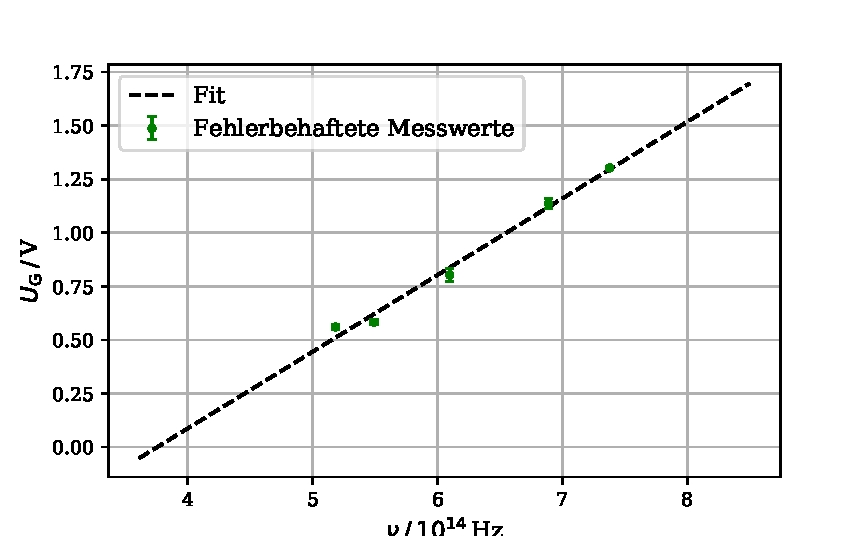
\includegraphics{grenz.pdf}
  \caption{Die berechneten Grenzspannungen gegen die Frequenzen der Spektrallinien sowie die Regressionsgerade.}
  \label{fig:grenz}
\end{figure}

Zuletzt wird das Verhalten des Photostroms der gelben Spektrallinie in einem größeren Intervall der Brems- bzw. Beschleunigungspannung
(-20 bis 20 V) untersucht. Die zugehörigen Messwerte befinden sich in Tabelle \ref{tab:gelb2}
und sind in Abbildung \ref{fig:gelb2} dargestellt.

\begin{figure}[H]
  \centering
  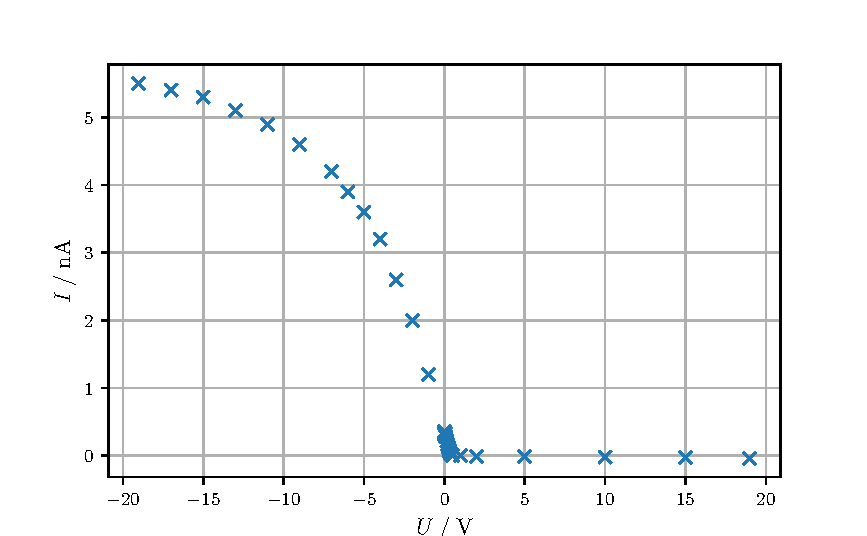
\includegraphics{gelb2.pdf}
  \caption{Der Photostrom beim Anlegen einer Brems- bzw. Beschleunigungsspannung bei gelbem Licht ($\lambda = \SI{578.05}{\nano\meter}$).}
  \label{fig:gelb2}
\end{figure}

\begin{table}[H]
  \centering
  \caption{Messwerte des Photostroms bei gelbem Licht ($\lambda = \SI{578.05}{\nano\meter}$) unter Anlegen einer Beschleunigungsspannung sowie einer Bremsspannung.}
  \label{tab:gelb2}
  \begin{tabular}{S[table-format=2.3] S[table-format=2.3] S[table-format=2.3] S[table-format=2.3]}
    \toprule
    {$U \:/\: \si{\volt}$} & {$I \:/\: \si{\nano\ampere}$} & {$U \:/\: \si{\volt}$} & {$I \:/\: \si{\nano\ampere}$}\\
    \midrule
-19   &  5.5 & 0.10 &   0.280     \\
-17   &  5.4 & 0.15 &   0.220     \\
-15   &  5.3 & 0.20 &   0.170     \\
-13   &  5.1 & 0.25 &   0.120     \\
-11   &  4.9 & 0.30 &   0.084     \\
-9    &  4.6 & 0.35 &   0.055     \\
-7    &  4.2 & 0.40 &   0.030     \\
-6    &  3.9 & 0.45 &   0.015     \\
-5    &  3.6 & 0.50 &   0.005     \\
-4    &  3.2 & 1    &   0.0     \\
-3    &  2.6 & 2    &   -0.004    \\ 
-2    &  2.0 & 5    &   -0.009    \\ 
-1    &  1.2 & 10   &   -0.02     \\
0     &  0.32 & 15   &   -0.03    \\
0.01  &  0.360 & 19   &   -0.038  \\   
0.05  &  0.330  & & \\  
  \end{tabular}
\end{table}